\newpage
\section{Primes \& Greatest/Lowest Common Divisors}

\begin{Def}[Greatest Common Divisor (GCD)]

    \label{def:gcd}

    For all $a,b\in\mathbb{Z}$,\\
    The \textit{greatest common divisor} of $a$ and $b$, is the largest positive integer dividing both $a$ and $b$.\\
    I.e., $d\in\mathbb{Z}: d\mid a$ and $d\mid b$, and \underline{$d$ is unique.}

    \noindent
    Denoted: $\gcd(a,b)$.
\end{Def}

\begin{Proof}[GCD Existence and Uniqueness]

    \label{theo:gcd_existence_uniqueness}

    Let $a,b\in\mathbb{Z}$, and $d=\gcd(a,b)$.\\
    \begin{itemize}
        \item  \textbf{Existence:} $d$ exists by the Well-Ordering Principle, 
        as it's greatest element in the set of common divisors of $a$ and $b$.
        \item \textbf{Uniqueness:} Let there be another GCD $d'\in\mathbb{Z}$ such that $d'\mid a$ and $d'\mid b$.\\
        Then, $d'\mid d$ and $d\mid d'$, so $d=\pm d'$ (\ref{theo:reflexive_divisibility}). GCD must be positive, so $d=d'$.
    \end{itemize}

   

\end{Proof}

\begin{theo}[GCD Ideal Linear Combination of $\mathbb{Z}$]

    \label{theo:gcd_ideal_linear_combination}

    For all \(a, b,d \in \mathbb{Z}\) and $d=\gcd(a,b)$: \(a\mathbb{Z} + b\mathbb{Z} = d\mathbb{Z}\)

\end{theo}

\begin{Proof}[GCD Ideal Linear Combination of $\mathbb{Z}$]

    \label{proof:gcd_ideal_linear_combination}

    Let $I:=a\mathbb{Z} + b\mathbb{Z}$. Then there exists $c\in Z$ such that $c\mathbb{Z} = I$ (\ref{theo:ideal_generator}). Then $a,b,c\in I$, are all
    positive integers. We will prove facts of $c$:
    \begin{itemize}
        \item \textbf{Common Divisor: }$a,b\in I$ and $c\mathbb{Z}=I$. So $a,b\in c\mathbb{Z}$. Then $c\mid a$ and $c\mid b$ (\ref{theo:ideal_properties}).
        \item \textbf{Linear Combination:} Since $c\in I$ and $a\mathbb{Z} + b\mathbb{Z} = I$. There exists some linear combination $\underline{as+bt=c}$ for some $s,t\in\mathbb{Z}$ (\ref{def:ideal_operations}).
        \item \textbf{Greatest Divisor} Let $a,b\in I$ be the products $a=a'c'$ and $b=b'c'$, where $a',b'\in\mathbb{Z}$.
              Then there's a linear combination $a'c'+b'c'=c'(a'+b')=c$. So $c\mid c'$, hence $c$ is the greatest common divisor of $a$ and $b$.
        \item \textbf{Uniqueness:} By Lemma (\ref{theo:gcd_existence_uniqueness}), $c$ is unique.
    \end{itemize}
\end{Proof}

\newpage

\noindent
This next theorem heavily relies on Definition (\ref{theo:ideal_properties}) and the previous Proof (\ref{theo:gcd_ideal_linear_combination}).
\begin{theo}[Element Linear Combinations of $\mathbb{Z}$]

    \label{theo:element_linear_combinations}

    For all \(a, b,d \in \mathbb{Z}\) and $d=\gcd(a,b)$:\\
    There exists some \(s, t \in \mathbb{Z}\), such that \(as + bt = r\) if and only if $d\mid r$.
        
\end{theo}


\begin{Proof}[Element Linear Combinations of $\mathbb{Z}$]

    Let $r\in\mathbb{Z}$, and $d=\gcd(a,b)$, we have
    
    \begin{center}
        \setlength{\tabcolsep}{4pt} % Adjust column separation
\renewcommand{\arraystretch}{1.2} % Adjust row separation

        \begin{tabular}{p{2cm} p{1cm} p{2cm} p{5.5cm}}
            $as + bt = r$ & $\Longleftrightarrow$ & $r \in a\mathbb{Z} + b\mathbb{Z}$ & (Ideal Multiplicative Closure (\ref{def:ideal_operations})) \\
            & $\Longleftrightarrow$ & $r \in d\mathbb{Z}$ & (GCD Linear Combination (\ref{theo:gcd_ideal_linear_combination})) \\
            & $\Longleftrightarrow$ & $d \mid r$ & (Property of Ideals (\ref{theo:ideal_properties})) \\
        \end{tabular}
    \end{center}
\end{Proof}
\begin{Note}
    \textbf{Note:} In $as + bt = r$, $s$ and $t$ are not unique, \underline{nor do they have to be positive}: Example (\ref{def:ideal_operations})
\end{Note}

\noindent
From above it follows that:

\begin{Def}[Reltively Prime]

    \label{def:relatively_prime}

    For all \(a, b \in \mathbb{Z}\), \(a\) and \(b\) are \textit{relatively prime} if \(\gcd(a, b) = 1\).\\
    
    \noindent
    Also known as a \underline{\textbf{coprime}.}

\end{Def}
I.e., given the equation $as + bt = r$ in (\ref{theo:element_linear_combinations}), if $r=1$, then $a$ and $b$ are coprime.\\

\textbf{Examples:}
\begin{itemize}
    \item $\gcd(6,9)=3$, so $6$ and $9$ are not coprime.
    \item $\gcd(6,7)=1$, so $6$ and $7$ are coprime.
\end{itemize}

\begin{Tip}
    It's crucial to understand the reasoning behind $as+bt=r$ and it's relation to ideals generated under $\mathbb{Z}$. I.e., understand ideals (\ref{def:ideal}), and their operations (\ref{def:ideal_operations}) robustly.
\end{Tip}

\newpage 

\begin{theo}[Cancellation of GCD]

    \label{theo:cancellation_of_gcd}

    Let \( a, b, c \in \mathbb{Z} \) such that \( c \mid ab \) and \( \gcd(a, c) = 1 \). Then \( c \mid b \).
\end{theo}

\begin{Proof}[Coprime Coefficient Divisibility]

    Let $a,b,c\in\mathbb{Z}$ such that $c\mid ab$ and $\gcd(a,c)=1$. $a$ and $c$ are coprime (\ref{def:relatively_prime}). Then there exists some $s,t\in\mathbb{Z}$
    such that $as+ct=1$ (\ref{theo:element_linear_combinations}).Then, 
    \begin{align*}
        as+ct=1 & \text{ (Given)}\\
        abs + cbt = b & \text{ (Multiply by $b$)}\\
        cds + cbt = b & \text{ (Sub. $ab$ as $c\mid ab\Rightarrow ab = cd,d\in\mathbb{Z}$)}\\
        c(ds+bt)=b & \text{ (Factor out $c$).}
    \end{align*}
    Yields $(ds+bt)\in\mathbb{Z}$, say $m$. So $cm = b$, hence $c\mid b$.
\end{Proof}

\begin{theo}[Euclid's Lemma]

    Let \( p \) be a prime, and \( a, b \in \mathbb{Z} \). If \( p \mid ab \), then \( p \mid a \) or \( p \mid b \).
\end{theo}

\begin{Proof}[Euclid's Lemma]

    \label{theo:euclids_lemma}

    Let $p$ be a prime, and $a,b\in\mathbb{Z}$ such that $p\mid ab$.
    \begin{itemize}
        \item If $p\mid a$, we satisfy the claim.
        \item If $p\nmid a$, then $\gcd(p,a)=1$ (\ref{def:prime_numbers}). So by Cancellation of GCD (\ref{theo:cancellation_of_gcd}), $p\mid b$.
    \end{itemize}
\end{Proof}
\begin{Note}
    \textbf{Note:} Primes only have two divisors: $1$ and itself. So if $p\nmid a$, then $\gcd(p,a)$ must be $1$.
\end{Note}
\begin{Tip}
    Euclid is pronounced ``You-clid''. He was a Greek mathematician who lived around 300 BC. His work laid the foundation for number theory.
    He primarily worked on the properties of prime numbers, and is known for his algorithm to find the GCD of two numbers.
\end{Tip}

\newpage

\noindent
Our most important theorem, \underline{\textbf{The Fundamental Theorem of Arithmetic}}:

\begin{theo}[Fundamental Theorem of Arithmetic (FTA)]

    \label{theo:FTA}

    Every $n\in\mathbb{Z}:n>1$ is prime or is product of primes, up to the order of the factors.
\end{theo}
By ``up to the order of the factors", we mean that the factorization is commutative.\\
\textbf{Example:} $30=2\cdot3\cdot5$ or $3\cdot2\cdot5$. The factorization is unique, except order (commutative).\\

\begin{Proof}[Fundamental Theorem of Arithmetic]

    Let $n\in\mathbb{Z}$ be a non-zero integer.\\

    \noindent
    \textbf{Existence:} by induction of $n$,
    \begin{itemize}
        \item \textbf{Base Case:} $n=2$, which holds as $2$ is prime.
        \item \textbf{Inductive Hypothesis:} Assume for all $n=k$, $k$ is prime or product of primes.
        \item \textbf{Inductive Step:} Let $n=k+1$. 
        \begin{itemize}
            \item If $n$ is prime, then we're done.
            \item $n$ is not prime, then $n=ab\in\mathbb{Z}$ where $a\leq b<n,$ otherwise $ab>n$. Reasoning:\\
                    If \( a \geq n \) or \( b \geq n \), then \( ab \geq n^2 \), contradicting \( ab = n \) unless \( n = 1 \), however \( n \geq 2 \).
            \item \textbf{Recursively:} Then $a$ and $b$ are prime or product of primes (Inductive Hypothesis). Then $n$ is a product of primes.
        \end{itemize}

        \noindent
        Therefore by induction, every $n\in\mathbb{Z}:n>1$ is prime or is product of primes.
    \end{itemize}
    
    \noindent
    \textbf{Uniqueness:} Let there be two different factorizations: $n = p_1p_2\ldots p_k= q_1q_2\ldots q_j$.\\
    Both factorizations are products of primes. We divide both sides by $p_1$:
    \begin{center}
        \begin{tabular}{cc}
            \(p_2p_3\ldots p_k = \dfrac{q_1q_2\ldots q_j}{p_1}\) &  \((p_1)(p_2\ldots p_k) = (q_1q_2\ldots q_j)\) \\
            (Simplified left side) & (Multiply by \(p_1\)) \\
       \end{tabular}
    \end{center}

    \noindent
    Let $m:=(p_1)$, $n:=(p_2\ldots p_k)$, $k:=(q_1q_2\ldots q_j)$. Then $mn=k$, so $m\mid k$. Take
    out $q_1$ from $k$, then $m\mid q_1\cdot k$. By Euclid's Lemma (\ref{theo:euclids_lemma}), $m\mid q_1$ or $m\mid k$ (the rest of the factors).
    \begin{itemize}
        \item If $m\mid q_1$, then $m=q_1$, by definition of prime (\ref{def:prime_numbers})
        \item If $m\mid k$, then $m$ equals some other prime in $k$.
    \end{itemize} 
    Continuing from $p_2$ to $p_k$ results in $p_i=q_i$ for all $i$, thus the factorization must be unique.
\end{Proof}

\newpage

\begin{theo}[Euclids Theorem]

    \label{theo:euclids_theorem}
    
        There are infinitely many primes.
\end{theo}

\begin{Proof}[Euclids Theorem]
    Say there are a finite number of primes: $p_1,p_2,\ldots,p_n$.\\
    Let $M:=p_1\times p_2\times\ldots\times p_n$ be the product of those primes. Let $N=M+1$:
    \begin{align*}
        N = M+1&\\
        N= p_1\times p_2\times\ldots\times p_n + 1&\\
        N= (p_1)(p_2\times\ldots\times p_n) + 1&\text{ (Form of Division Alg. (\ref{theo:division_algorithm}))}\\
    \end{align*}
    $N$ has remainder 1 when divided by any such prime. Thus, $N$ is not a product of primes.\\
    Then $N$ must be a prime (\ref{theo:FTA}).
\end{Proof}

\noindent
Extending the the Fundamental Theorem of Arithmetic (\ref{theo:FTA}):
\begin{theo}[FTA Corollary]

    \label{theo:FTA_corollary}

    Every $n\in\mathbb{Z}:n>1$ has a unique prime factorization, up to order \underline{and sign}:
    \[n = \pm p_1^{e_1}p_2^{e_2}\ldots p_k^{e_k}\]
    For $p_1,p_2,\ldots,p_k$ distinct primes, and $e_1,e_2,\ldots,e_k$ positive integers.
\end{theo}

\begin{Proof}[FTA Corollary]

   Let $n\in\mathbb{Z}:n>3$ and a composite number.
   \begin{itemize}
    \item $n=ab\in\mathbb{Z}$ by definition of a composite (\ref{def:composite_numbers}).
    \item Then $a$ and $b$ are prime or product of primes (\ref{theo:FTA}).
    \item Let $a$ and $b$ be prime and $a=b$
   \end{itemize}
  
   \noindent
   Then $n=a^2$, a prime squared.
\end{Proof}

\newpage
\noindent
We'll begin to define functions---which may or may not have logic---to abstract concepts.
\begin{Func}[Prime Exponents - $\mathcal{V}_p(n)$]

    For each prime $p$ where $n=p^em \in\mathbb{Z}$ and $p\nmid m$. We define $\mathcal{V}_p(n)=e$.\\
    I.e., $\mathcal{V}_p(n)$ is the exponent of $p$ in the prime factorization of $n$. 
\end{Func}
In specifying $p\nmid m$, we ensure that $p^e$ is the highest power of $p$ dividing $n$.\\

\noindent
We'll use this to abstract the Fundamental Theorem of Arithmetic further:
\begin{theo}[FTA Abstracted by $\mathcal{V}_p(n)$]

    \label{theo:FTA_abstracted}

    Every $n\in\mathbb{Z}:n>1$ has a unique prime factorization, up to order and sign:
    \LARGE \[n = \pm \prod_{p} p^{\mathcal{V}_p(n)}\]
    
    \normalsize
    \noindent
    For $p$ distinct primes.
\end{theo}
\begin{Note}
    \textbf{Note:} The notation $\prod$ is to products, as $\sum$ is to sums.
\end{Note}

\noindent
To expand our theorem for clarity:
\LARGE
\[
    n = \pm \prod_{p} p^{\mathcal{V}_p(n)} = \pm p_1^{\mathcal{V}_{p_1}(n)} p_2^{\mathcal{V}_{p_2}(n)} \cdots p_k^{\mathcal{V}_{p_k}(n)}
\]
\normalsize

\noindent
The ``$\pm$'' accounts for the sign of $n$. Say $n=-30$, then $n=-(2\cdot3\cdot5)$.\\

\noindent
The function $\mathcal{V}_p(n)$ help us generalize GCD and \underline{\textbf{Least Common multiple} (LCM),} but first we define two other functions:

\begin{Func}[Minumum \& Maximum - $\min()$, $\max()$]
    
        For all $a,b\in\mathbb{Z}$,
        \begin{itemize}
            \item $\min(a,b)$ is the smallest of $a$ and $b$.
            \item $\max(a,b)$ is the largest of $a$ and $b$.
        \end{itemize}
\end{Func}

\newpage

\begin{theo}[Operations of $\mathcal{V}_p(n)$]

    \label{theo:operations_of_V_p(n)}

    For all $a,b\in\mathbb{Z}$ and $p$ prime:
    \begin{itemize}
        \item $\mathcal{V}_p(ab) = \mathcal{V}_p(a) + \mathcal{V}_p(b)$
        \item $\mathcal{V}_p(a^k) = k \mathcal{V}_p(a)$
        \item $a \mid b \iff \mathcal{V}_p(a) \leq \mathcal{V}_p(b) \text{ for all primes } p$
    \end{itemize}
\end{theo}

\begin{Proof}[Operations of $\mathcal{V}_p(n)$]
    For all $a,b\in\mathbb{Z}$ and $p$ prime:
    \begin{itemize}
        \item \underline{$\mathcal{V}_p(ab) = \mathcal{V}_p(a) + \mathcal{V}_p(b)$.}\\
        Let $a = p^e m$ and $b = p^{e'} m'$, where $p \nmid m$ and $p \nmid m'$. 

        \vspace{-.5em}
        \begin{itemize}
            \item $ab = p^e m \times p^{e'} m' = p^{e + e'} m m'$
            \item $\mathcal{V}_p(ab) = e + e' = \mathcal{V}_p(a) + \mathcal{V}_p(b)$
        \end{itemize}
        \vspace{.5em}

        \item \underline{$\mathcal{V}_p(a^k) = k \mathcal{V}_p(a)$.}\\
        Let $a = p^e m$, where $p \nmid m$.

        \vspace{-.5em}
        \begin{itemize}
            \item $a^k = (p^e m)^k = p^{ke} m^k$
            \item $\mathcal{V}_p(a^k) = ke = k \mathcal{V}_p(a)$
        \end{itemize}
        \vspace{.5em}

        \item \underline{$a \mid b \iff \mathcal{V}_p(a) \leq \mathcal{V}_p(b) \text{ for all primes } p$.}\\
        Let $a = p^e m$ and $b = p^{e'} m'$, where $p \nmid m$ and $p \nmid m'$. 
        \vspace{-.5em}
        \begin{itemize}
            \item If $a \mid b$, then $b = aq\in\mathbb{Z}$. Thus, $\mathcal{V}_p(a) \leq \mathcal{V}_p(b)$, i.e., $e\leq e'$, otherwise $b<aq$.
            \item $\mathcal{V}_p(a) \leq \mathcal{V}_p(b)$, both refer to $p$. Thus $a\mid b$ as $a$ can pull some factor $p^e$ out of $b$.
        \end{itemize}
    \end{itemize}
\end{Proof}

\begin{Tip}
    Remember that $\mathcal{V}_p(n)$ is some arbitrary function we defined.
    Despite this function being \textit{made-up}, it has very \textbf{real} implications as we'll see in the next theorem. 
    It helps to abstract concepts, to avoid repetition and the accumulation of details.\\

    \noindent
    Similar to how computers are built on binary logic, and then subsequently written in some
    abstracted higher-level language. Then even those languages have their own abstractions through various libraries and frameworks,
    all helping speed up the process of development.

\end{Tip}

\newpage

\begin{theo}[GCD abstracted by $\mathcal{V}_p(n)$]

    \label{theo:GCD_abstracted}

    For all $a,b\in\mathbb{Z}$:
    \[\gcd(a,b) = \prod_{p} p^{\min(\mathcal{V}_p(a),\mathcal{V}_p(b))}\]

\end{theo}

\begin{Proof}[GCD abstracted by $\mathcal{V}_p(n)$]

    \label{proof:gcd_abstracted}

    The $\gcd(a,b) = \prod_{p} p^{\min(\mathcal{V}_p(a),\mathcal{V}_p(b))}$ can be visualized into the following:
    \[
    \begin{array}{ccc|c|c|c|c}
    
    a=&\prod&p_1^{e_1} & p_2^{e_2} & p_3^{e_3} & \dots & p_k^{e_k} \\
    b=&\vdots&p_1^{e'_1} & p_2^{e'_2} & p_3^{e'_3} & \dots & p_k^{e'_k} \\
    \hline
    gcd(a,b)=&\vdots&p_1^{\min(e_1, e'_1)} & p_2^{\min(e_2, e'_2)} & p_3^{\min(e_3, e'_3)} & \dots & p_4^{\min(e_k, e'_k)} \\

    \end{array}
    \]

    \noindent
    Separating $a$ and $b$ into their prime factors, taking the minimum exponent of each pair $p_i$,
    effectively striping all unnecessary factors, leaving only and all common factors between them.\\
    
    \noindent
    I.e., the GCD.

\end{Proof}

\begin{Def}[Least Common Multiple (LCM)]

    For all $a,b,n\in\mathbb{Z}$\\
    The smallest positive integer divisible by both $a$ and $b$ is the \textit{least common multiple}.\\
    I.e., $n$ is the smallest such integer that $a\mid n$ and $b\mid n$. \underline{$n$ is unique.}\\

    \noindent
    Denoted: $\lcm(a,b)$.
\end{Def}


\begin{Proof}[LCM Existence and Uniqueness]

    \label{proof:lcm_existence_uniqueness}

    Let $a,b\in\mathbb{Z}$, and $m=\text{lcm}(a,b)$, $m$ is the largest such integer that $a\mid m$ and $b\mid m$.
    \begin{itemize}
        \item  \textbf{Existence:} $m$ exists by the Well-Ordering Principle.
        \item \textbf{Uniqueness:} Let there be another smallest $m'\in\mathbb{Z}:a\mid m'$ and $b\mid m'$.\\
        Then, both $m$ and $m'$ are divisible by $a$ and $b$, it follows that $m \mid m'$ and $m' \mid m$.\\
        Thus, $m=\pm m'$ (\ref{theo:reflexive_divisibility}). LCM must be positive, so $m = m'$.
    \end{itemize}
\end{Proof}

\newpage

\begin{theo}[LCM abstracted by $\mathcal{V}_p(n)$]

    \label{theo:LCM_abstracted}

    For all $a,b\in\mathbb{Z}$:
    \[\lcm(a,b) = \prod_{p} p^{\max(\mathcal{V}_p(a),\mathcal{V}_p(b))}\]
\end{theo}

\begin{Proof}[LCM abstracted by $\mathcal{V}_p(n)$]

    \label{proof:lcm_abstracted}

    The $\lcm(a,b) = \prod_{p} p^{\max(\mathcal{V}_p(a),\mathcal{V}_p(b))}$ can be visualized into the following:
    \[
    \begin{array}{ccc|c|c|c|c}
    
    a=&\prod&p_1^{e_1} & p_2^{e_2} & p_3^{e_3} & \dots & p_k^{e_k} \\
    b=&\vdots&p_1^{e'_1} & p_2^{e'_2} & p_3^{e'_3} & \dots & p_k^{e'_k} \\
    \hline
    lcm(a,b)=&\vdots&p_1^{\max(e_1, e'_1)} & p_2^{\max(e_2, e'_2)} & p_3^{\max(e_3, e'_3)} & \dots & p_4^{\max(e_k, e'_k)} \\

    \end{array}
    \]

    \noindent
    Separating $a$ and $b$ into their prime factors, taking the maximum exponent of each pair $p_i$,
    effectively including only and all necessary factors between them.\\
    
    \noindent
    I.e., the LCM.
\end{Proof}

\begin{theo}[GCD-LCM Relationship]

    \label{theo:gcd_lcm_relationship}

    For all $a,b\in\mathbb{Z}$:
    \[\gcd(a,b)\cdot\lcm(a,b) = |ab|\]
    which follows:
    \LARGE \[lcm(a,b) = \dfrac{|ab|}{\gcd(a,b)}\]
\end{theo}

\begin{center}
    \textit{Proof on next page.}
\end{center}

\newpage

\begin{Proof}[GCD-LCM Relationship]

    \label{proof:gcd_lcm_relationship}

    Between $a,b\in\mathbb{Z}$: 
    \begin{itemize}
        \item GCD is the largest common factor.
        \item LCM is the smallest common multiple.
    \end{itemize}

    We visualize this relationship:
    
    \begin{center}
    
        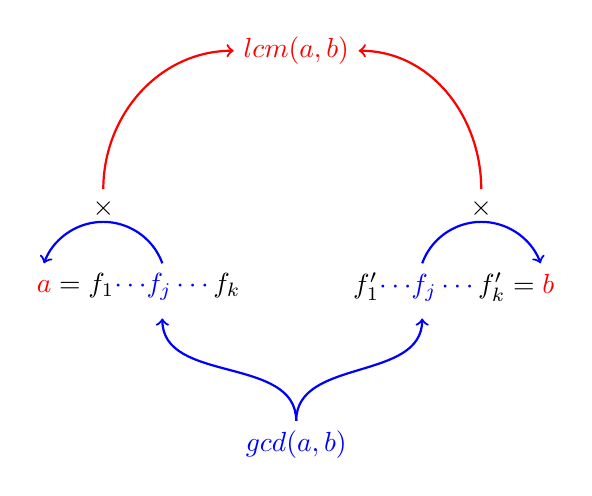
\begin{tikzpicture}
            % Nodes
            \node (lcm) at (0,3) {\textcolor{red}{$\text{lcm}(a,b)$}};
            
            \node (a) at (-2,0) {$\color{red}a\color{black} = f_1\color{blue}{\cdots}f_j\cdots\color{black} f_k$};
            \node (b) at (2,0) {$f_1' \color{blue}{\cdots}f_j\cdots \color{black} f_k'=\color{red}b$};
            
            \node (gcd) at (0,-2) {\textcolor{blue}{$\text{gcd}(a,b)$}};
            
           
            
            \draw[->, blue, thick] (gcd) to [out=90,in=-90] (-1.7,-.4);
            \draw[->, blue, thick] (gcd) to [out=90,in=-90] (1.6,-.4);

            % blue crosses times
            \draw[->, blue, thick] (-1.7,.3)  arc
            [
                start angle=20,
                end angle=160,
                x radius=.8cm,
                y radius =0.8cm
            ];
            \draw[->, blue, thick] (1.6,.3) arc
            [
                start angle=160,
                end angle=20,
                x radius=.8cm,
                y radius =0.8cm
            ];

            % Times
            \node (timesa) at (-2.45,1) {{$\times$}};
            \node (timesb) at (2.35,1) {{$\times$}};
            
            % blue crosses
             \draw[->, red, thick] (timesa) to [out=90,in=180]  (lcm);
             \draw[->, red, thick] (timesb) to [out=90,in=0] (lcm);
        
        \end{tikzpicture}
    \end{center}
    Let $f_1,f_2,\ldots,f_k:=a$'s factors, $f_1',f_2',\ldots,f_k':=b$'s factors. Let $\gcd(a,b):=f_j$, factors $a\cap b$.
    
    

    % \begin{align*}
    %     \lcm(a,b) = abc\in\mathbb{Z} & \text{ As ($ab\mid\lcm(a,b)$ (\ref{def:division}))}\\


    % \end{align*}
    
    \end{Proof}






